\section{Semantic segmentation with a compact U-Net (SmallUNet)}
\label{sec:moon_recognition}

Complementing the instance formulation, the same terrain is addressed as dense, pixel-level labelling: multi-label semantic segmentation, with seven independent binary classifications per pixel (Sect.~\ref{sec:mr_dataset}), posed per class rather than as a single-label softmax problem because classes can coexist in a pixel.

\paragraph{Pre-processing.}
Each grayscale tile is converted into a three-channel tensor providing complementary views of the same image: (i) min-max normalised intensity; (ii) CLAHE (\texttt{skimage} \texttt{equalize\_adapthist}, clip limit 0.03) to enhance local contrast; (iii) the Sobel gradient magnitude, highlighting boundaries and ridge-like structures. Because CLAHE costs ${\sim}3$\,s per tile on CPU, all tensors are precomputed once and cached as compressed \texttt{.npz} files.

\paragraph{Architecture.}
SmallUNet follows the U-Net encoder--decoder paradigm \citep{ronneberger2015unet} at reduced scale: three \emph{Down} blocks ($2\times2$ max-pooling + DoubleConv, i.e.\ two $3\times3$ convolution--BatchNorm--ReLU stages), a symmetric decoder using transposed convolutions and skip-connection concatenation, and a $1\times1$ output head mapping 32 channels to 7 independent logit maps. Two optional components are studied below: residual (ResNet-style) shortcuts inside each DoubleConv block, and spatial Dropout2d at the bottleneck. The base width $w$ scales the channel progression ($w$--$8w$): $w=16/32/64$ gives 0.51M/2.0M/8.0M parameters.

\paragraph{Losses and training.}
Two composite losses are compared: \emph{BCEDice} (binary cross-entropy plus soft Dice, macro-averaged over classes) and \emph{FocalDice}, which replaces BCE with the binary focal loss \citep{lin2017focal} ($\gamma=2$, $\alpha=0.25$) and weights the per-class Dice terms $[1,4,5,5,5,5,5]$ to penalise misdetection of rare classes. Unless noted otherwise, the definitive experiments ran on an NVIDIA Tesla T4 (CloudVeneto) on the full 15{,}931-tile dataset for 30 epochs (batch 16, Adam, cosine annealing $10^{-3}\!\to\!10^{-5}$); local Apple-Silicon runs served for prototyping. Validation is computed every epoch: per-class precision, recall, F1, IoU at $\tau=0.5$, plus threshold-free AP.

\subsection{Ablation campaign}
\label{sec:mr_augmentation}

Three controlled studies were run in sequence; Table~\ref{tab:final_summary} collects the best result of each, and Appendix~\ref{app:unet} the architecture details, loss definitions, full per-study tables, and validation curves.

\paragraph{Study 1 --- architecture.}
Five cumulative configurations (BCEDice; FocalDice; +residual; +dropout $p=0.3$; +both) were compared on the full T4 protocol. Residual shortcuts consistently improve aggregate F1, IoU, and AP; dropout alone does not help, likely because sparse labels already regularise the network; the combination \textbf{+both} is best (mean F1 0.2076, mean AP 0.2004, ridge AP 0.453). Crater AP is uniformly high (0.939--0.951) across all configurations, but against the 0.821 prevalence baseline of Table~\ref{tab:prevalence} this is only a modest lift over chance: architecture matters primarily for rare, structurally subtle classes such as ridges, where AP ${\sim}0.45$ is ${\sim}70\times$ the 0.0064 chance level.

\paragraph{Study 2 --- width.}
Sweeping $w\in\{16,32,64\}$ under the best architecture shows strong diminishing returns: the wide model is best (mean AP 0.2016, mean F1 0.2153) but improves on $w=32$ by only $+0.0006$ mean AP at $4\times$ the parameters and $2.3\times$ the epoch time, and the 505K-parameter $w=16$ model lands within 0.001 mean AP of the 8M-parameter one --- the most parameter-efficient option for constrained deployment.

\paragraph{Study 3 --- augmentation.}
The most striking result: training \emph{without} geometric augmentation (random flips and $90\degree/180\degree/270\degree$ rotations) beats the augmented model on every metric --- mean AP 0.2647 vs 0.2027, ridge AP 0.558 vs 0.457. Two effects can combine here. Geologically, Marius Hills has a strong directional bias --- ridges and rilles follow the regional stress field, and the Sun azimuth is consistent within the mosaic --- so flips and rotations inject orientations and shading that are physically absent, violating the assumption that transformed inputs remain representative \citep{shorten2019augmentation}; rotationally symmetric craters are indeed unaffected (AP 0.947 vs 0.942). Methodologically, however, the random tile split leaks overlapping pixels into validation (Sect.~\ref{sec:splits}), and a non-augmented model is freer to memorise tile appearance --- a leaky split rewards exactly that. To separate the two effects the pair was re-trained under the leakage-free spatial split, as a scaled paired protocol on local hardware (10{,}000 tiles, 30 epochs, identical seeds and schedule in both arms; Table~\ref{tab:spatial_rerun}, Fig.~\ref{fig:spatial_rerun}). The conclusion survives: no-augmentation stays ahead at every epoch. The decomposition is instructive --- absolute scores drop sharply (ridge AP 0.558 $\to$ 0.385, confirming that random-split numbers were inflated by memorisation) and the aggregate gap narrows (mean AP $+0.014$ vs $+0.062$), but for the direction-sensitive ridge class a large genuine gap persists (AP 0.385 vs 0.306 on strictly disjoint pixels), exactly the signature predicted by the geological explanation.

\begin{table}[htbp]
\centering
\caption{Best result from each ablation study (full T4 protocol, 30 epochs; random tile split).}
\label{tab:final_summary}
\resizebox{\columnwidth}{!}{%
\begin{tabular}{llrrrr}
\toprule
Study & Best config & Params & Mean F1 & Mean AP & Ridge AP \\
\midrule
Architecture & +both ($w=32$, augmented) & 2.0M & 0.2076 & 0.2004 & 0.453 \\
Width        & wide ($w=64$, augmented)  & 8.0M & 0.2153 & 0.2016 & 0.445 \\
Augmentation & +both, $w=32$, \textbf{no aug} & 2.0M & \textbf{0.2986} & \textbf{0.2647} & \textbf{0.558} \\
\bottomrule
\end{tabular}
}
\end{table}

\begin{table}[htbp]
\centering
\caption{Augmentation ablation under the leakage-free spatial split (10{,}000 tiles, 30 epochs, paired arms). \texttt{candidate\_rille} has zero positive pixels in the spatial validation set and is excluded from the macro averages.}
\label{tab:spatial_rerun}
\resizebox{\columnwidth}{!}{%
\begin{tabular}{lrrrr}
\toprule
Config & Mean F1 & Mean AP & Ridge F1 & Ridge AP \\
\midrule
\textbf{no augmentation} & \textbf{0.2294} & \textbf{0.2239} & \textbf{0.4586} & \textbf{0.3847} \\
+augmentation            &        0.2208  &        0.2096  &        0.3970  &        0.3060  \\
\bottomrule
\end{tabular}
}
\end{table}

\begin{figure}[htbp!]
\centering
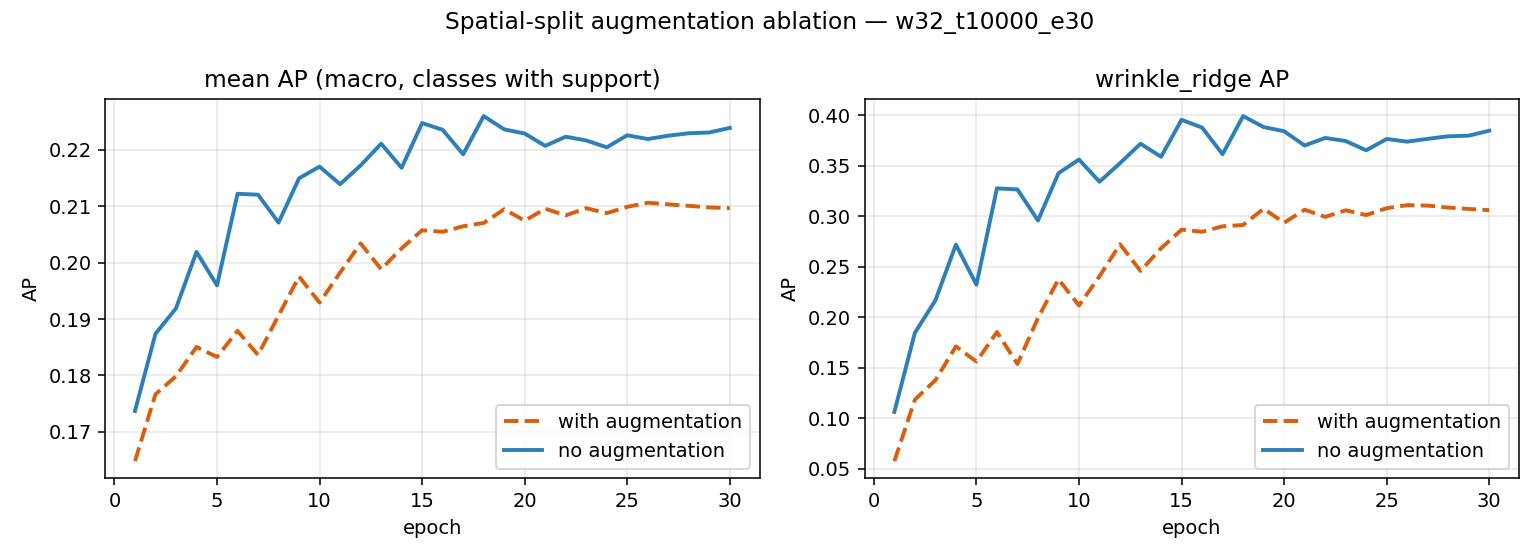
\includegraphics[width=0.85\columnwidth,keepaspectratio]{figures/MR/spatial_w32_t10000_e30_val_ap.png}
\caption{Validation AP across training epochs under the leakage-free spatial split (macro mean over classes with support, left; \texttt{wrinkle\_ridge}, right). The no-augmentation arm dominates at every epoch on both metrics.}
\label{fig:spatial_rerun}
\end{figure}

\paragraph{Definitive model.}
The definitive model is SmallUNet with $w=32$, FocalDice, residual shortcuts, bottleneck dropout ($p=0.3$), trained \emph{without} augmentation for 30 epochs on the full dataset. One caveat applies to this synthesis across studies: Studies 1--2 were run with augmentation enabled, before Study 3 established it is harmful; their selected components are architectural choices not expected to interact strongly with augmentation, but re-confirming those rankings in the no-augmentation regime remains the natural next experiment.

\subsection{Qualitative evaluation}
\label{sec:mr_qualitative}

Metrics alone do not reveal \emph{how} a model fails, so the ablations are complemented by a visual comparison on identical validation tiles for the BCEDice baseline and the definitive model. The ridge comparison (Fig.~\ref{fig:qualitative_ridge}) shows that the metric gains of the definitive model correspond to a real, visible improvement in the completeness of the recovered ridge network, with errors concentrated on thin, low-contrast segments. The crater comparison (Fig.~\ref{fig:qualitative_crater}), conversely, makes the saturation argument of Sect.~\ref{sec:mr_dataset} concrete: the ground truth fills entire tiles, so predicting ``everywhere'' is trivially correct.

\begin{figure}[htbp!]
\centering
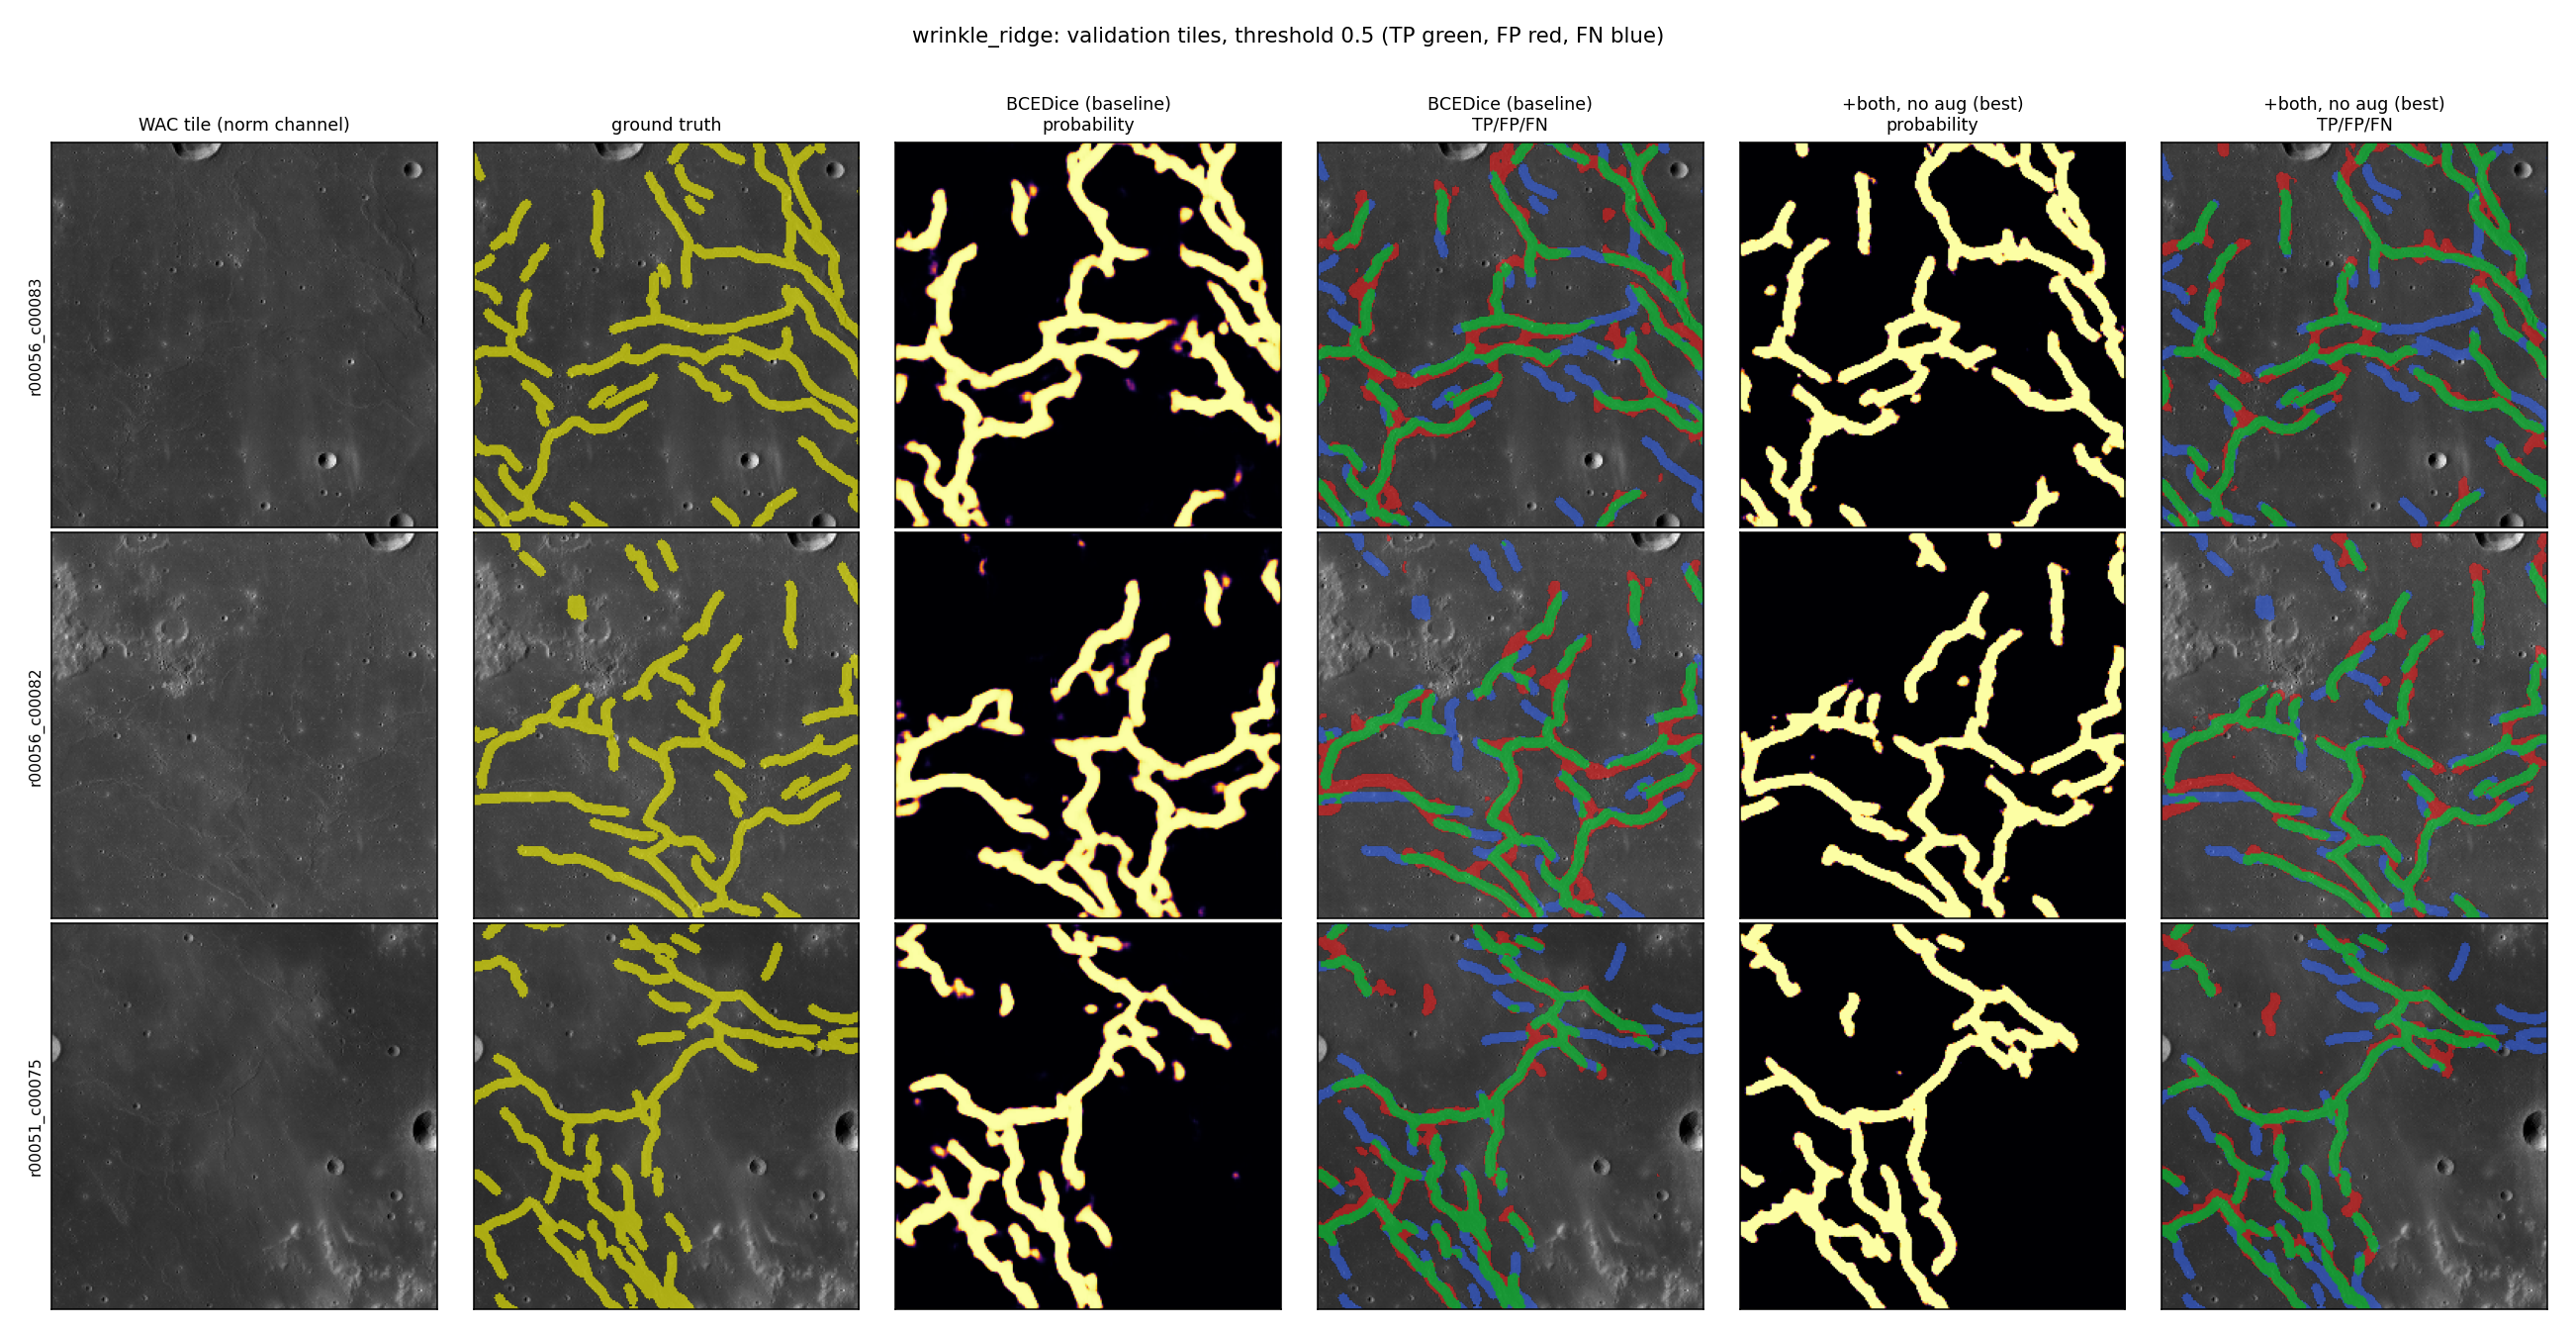
\includegraphics[width=0.85\columnwidth,keepaspectratio]{figures/MR/qualitative_wrinkle_ridge.png}
\caption{Wrinkle-ridge qualitative comparison on three validation tiles (TP green, FP red, FN blue). Both models recover the topology of the ridge network; the definitive model (+both, no augmentation) produces visibly more complete coverage and fewer false positives than the BCEDice baseline.}
\label{fig:qualitative_ridge}
\end{figure}

\begin{figure}[htbp!]
\centering
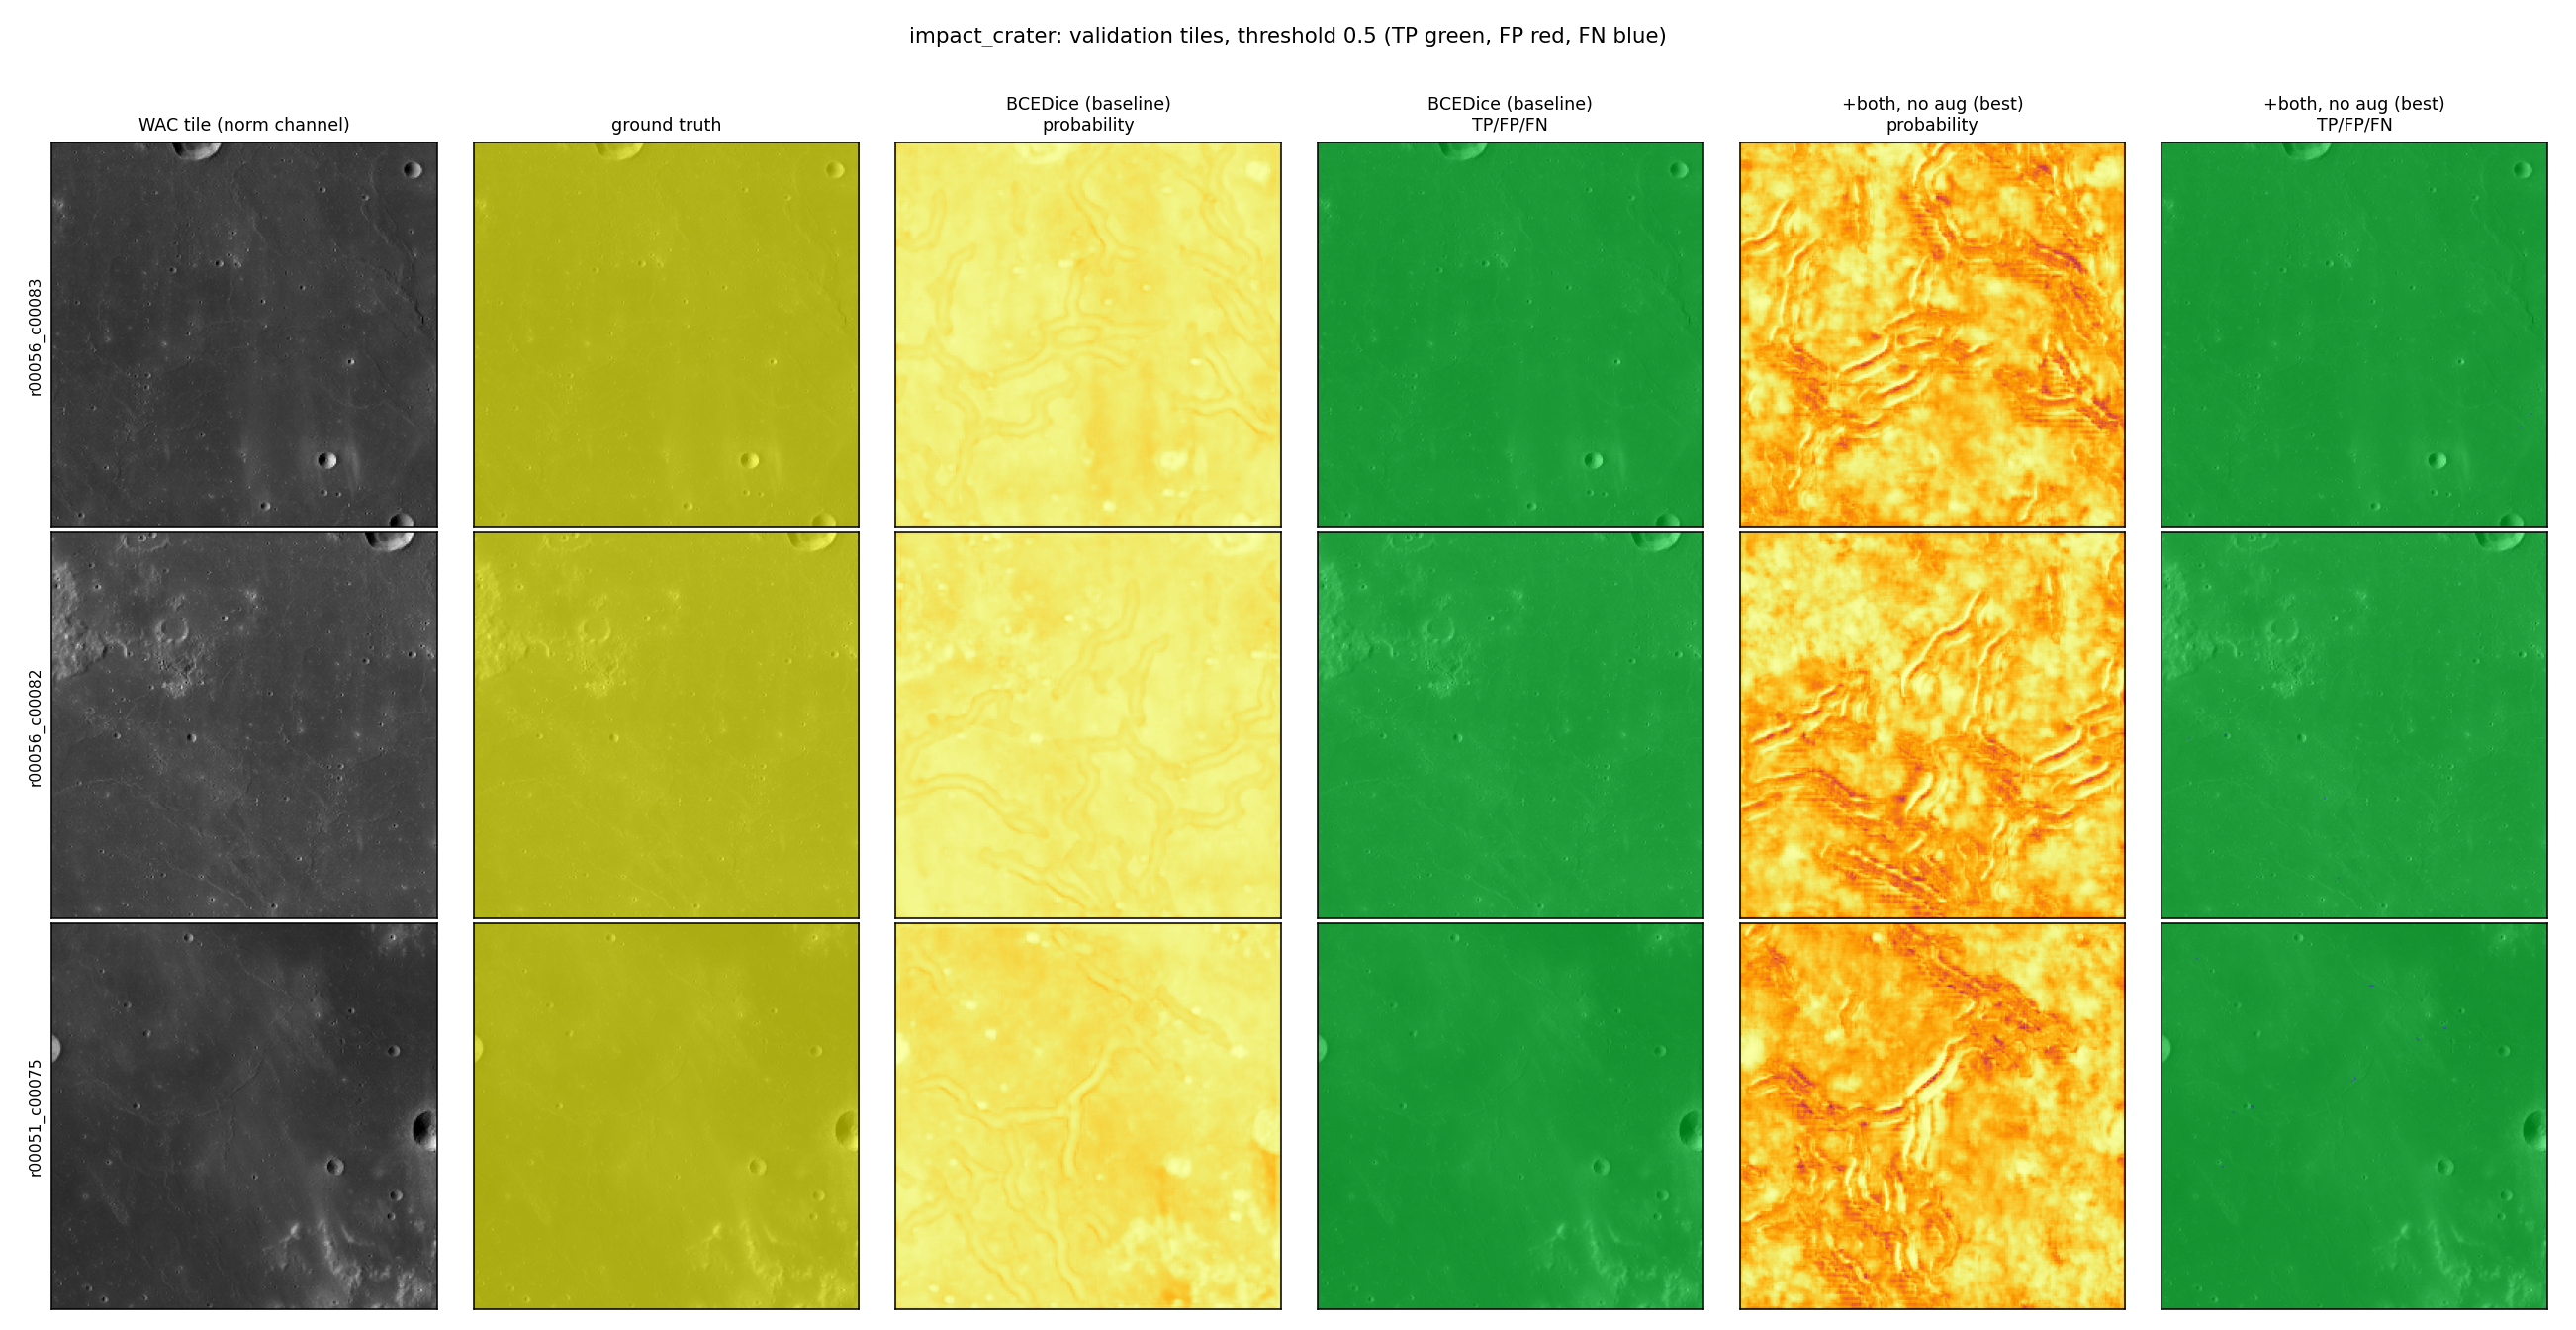
\includegraphics[width=0.85\columnwidth,keepaspectratio]{figures/MR/qualitative_impact_crater.png}
\caption{Impact-crater qualitative comparison on the same tiles. The ground truth covers the \emph{entire} tile (cf.\ the 82.1\% pixel prevalence and 50.7\% fully-covered tiles of Table~\ref{tab:prevalence}), so a prediction of ``everywhere'' is trivially correct: direct visual evidence that the crater channel behaves as a near-coverage layer and that crater AP must be read against its 0.821 chance baseline.}
\label{fig:qualitative_crater}
\end{figure}
